\chapter{Extend's Internal Architecture}

\begin{center}
  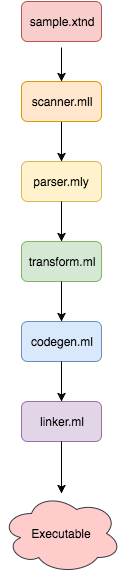
\includegraphics[width=.20\textwidth, height=15cm]{img/Execution.png}
\end{center}

\newpage

\section{The Extend Compiler}
The Extend compilation process consists of several source files, each of which performs a different function in the compilation pipeline.

\begin{itemize}
  \item \texttt{scanner.mll}: OCamllex scanner - consumes tokens.
  \item \texttt{parser.mly}: OCamlyacc parser - represents the Extend grammar.
  \item \texttt{ast.ml}: Abstract Syntax Tree, created from the output of the parser and representing the structure of an Extend program.
  \item \texttt{transform.ml}: Performs syntactic desugaring for easier compilation.
  \item \texttt{semant.ml}: Analyzes the semantics of the program to ensure that the program adheres to the rules of the language.
  \item \texttt{codegen.ml}: The LLVM IR code generator.
  \item \texttt{linker.ml}: Calls intermediary compilation steps on the generated \texttt{.ll}, including external functions if needed.
\end{itemize}

  \subsection{The Scanner}
  The function of \texttt{scanner.mll} is to parse a text stream into various tokens to be used in an Extend program.
  Only the tokens that are valid in Extend are to be given to the parser; all others will return a syntax error marked by the line and character number.

  \subsection{The Parser and Abstract Syntax Tree}
  The parser converts the tokens read by the scanner into a syntax tree deemed acceptable grammar within the Extend Language. This is converted into an Abstract Syntax Tree, which has nodes that can be consumed by the back end of the Extend compiler.

  \subsection{The Transformer}
  The transformer expands compact statements in the Extend syntax tree into statements with equivalent functionality, but reduced breadth. This step is done to preserve the convenience for the user, but revert the code later into a form that is easier for the compiler to chew on.

  \subsection{The Semantic Analyzer}
  The semantic analyzer ensures that Extend functions, variables, expressions, and more are being used properly at compile time, and throws flavorful exceptions to the user so that they may better understand why their program was illegal.

  \subsection{The Code Generator}
  Provided that the program was deemed legal by \texttt{transform.ml}, the code generator will take the program definition in the abstract syntax tree and generate the appopriate LLVM IR to turn it into a functional program. Instructions to allocate memory, interact with external functions, and platform optimization can be found here.

  \subsection{The Linker}
  If successful LLVM IR is generated, the linker will adopt the role of building an executable object from the \texttt{.ll} file. This includes compiling it to an object file and linking the runtime environment along with other imported libraries.
